\documentclass[12pt, a4paper]{article}

%% ── Geometry ────────────────────────────────────────────────────────────────
\usepackage[a4paper, top=2.5cm, bottom=2.5cm,
            left=2.8cm, right=2.8cm, headheight=15pt]{geometry}

%% ── Fonts & encoding ────────────────────────────────────────────────────────
\usepackage[T1]{fontenc}
\usepackage[utf8]{inputenc}
\usepackage{palatino}
\usepackage{mathpazo}
\usepackage{microtype}

%% ── Mathematics ─────────────────────────────────────────────────────────────
\usepackage{amsmath, amssymb, amsthm, mathtools}
\usepackage{cancel}

%% ── Graphics & colour ───────────────────────────────────────────────────────
\usepackage{xcolor}
\usepackage{tikz}
\usetikzlibrary{arrows.meta, positioning, calc,
                decorations.pathreplacing, backgrounds, patterns, intersections}
\usepackage{pgfplots}
\pgfplotsset{compat=1.15}

%% ── Tables ──────────────────────────────────────────────────────────────────
\usepackage{booktabs, array, colortbl, multirow, tabularx}
\renewcommand{\arraystretch}{1.45}

%% ── Lists ───────────────────────────────────────────────────────────────────
\usepackage{enumitem}
\setlist[itemize]{leftmargin=1.8em, itemsep=3pt, topsep=4pt}
\setlist[enumerate]{leftmargin=1.8em, itemsep=3pt, topsep=4pt}

%% ── Callout boxes ───────────────────────────────────────────────────────────
\usepackage[most]{tcolorbox}
\tcbuselibrary{skins, breakable, theorems}

%% ── Headers, footers, TOC, captions ────────────────────────────────────────
\usepackage{fancyhdr}
\usepackage{lastpage}
\usepackage{tocloft}
\usepackage{caption}
\usepackage{float}

%% ── Hyperlinks ──────────────────────────────────────────────────────────────
\usepackage[colorlinks=true, linkcolor=navy,
            urlcolor=navy, citecolor=navy]{hyperref}

%% ── Spacing ─────────────────────────────────────────────────────────────────
\usepackage{parskip}
\setlength{\parskip}{6pt}
\setlength{\parindent}{0pt}

%% ═══════════════════════════════════════════════════════════════════════════
%%  COLOUR PALETTE
%% ═══════════════════════════════════════════════════════════════════════════
\definecolor{navy}{RGB}{10, 40, 105}
\definecolor{navylight}{RGB}{230, 237, 252}
\definecolor{gold}{RGB}{175, 128, 8}
\definecolor{lightgold}{RGB}{254, 248, 218}
\definecolor{teal}{RGB}{8, 108, 98}
\definecolor{lightteal}{RGB}{222, 248, 243}
\definecolor{crimson}{RGB}{148, 18, 28}
\definecolor{lightcrimson}{RGB}{255, 234, 234}
\definecolor{purple}{RGB}{78, 28, 132}
\definecolor{lightpurple}{RGB}{244, 237, 255}
\definecolor{solgreen}{RGB}{8, 92, 48}
\definecolor{lightsol}{RGB}{225, 252, 236}
\definecolor{charcoal}{RGB}{36, 36, 36}
\definecolor{slate}{RGB}{72, 84, 100}
\definecolor{tabhead}{RGB}{10, 40, 105}
\definecolor{tabeven}{RGB}{230, 237, 252}
\definecolor{orange}{RGB}{195, 90, 10}
\definecolor{lightorange}{RGB}{255, 242, 225}

%% ═══════════════════════════════════════════════════════════════════════════
%%  TCOLORBOX ENVIRONMENTS
%% ═══════════════════════════════════════════════════════════════════════════

\newtcolorbox{defbox}[1]{%
  breakable, enhanced,
  colback=navylight, colframe=navy, coltitle=white,
  fonttitle=\bfseries\sffamily, title={Definition\quad#1},
  arc=4pt, boxrule=1pt, left=8pt, right=8pt, top=6pt, bottom=6pt,
  attach boxed title to top left={yshift=-2mm, xshift=6mm},
  boxed title style={colback=navy, arc=3pt, boxrule=0pt}}

\newtcolorbox{thmbox}[1]{%
  breakable, enhanced,
  colback=lightteal, colframe=teal, coltitle=white,
  fonttitle=\bfseries\sffamily, title={Theorem\quad#1},
  arc=4pt, boxrule=1pt, left=8pt, right=8pt, top=6pt, bottom=6pt,
  attach boxed title to top left={yshift=-2mm, xshift=6mm},
  boxed title style={colback=teal, arc=3pt, boxrule=0pt}}

\newtcolorbox{propbox}[1]{%
  breakable, enhanced,
  colback=lightteal, colframe=teal, coltitle=white,
  fonttitle=\bfseries\sffamily, title={Proposition\quad#1},
  arc=4pt, boxrule=1pt, left=8pt, right=8pt, top=6pt, bottom=6pt,
  attach boxed title to top left={yshift=-2mm, xshift=6mm},
  boxed title style={colback=teal, arc=3pt, boxrule=0pt}}

\newtcolorbox{keybox}[1]{%
  breakable, enhanced,
  colback=lightgold, colframe=gold, coltitle=white,
  fonttitle=\bfseries\sffamily, title={#1},
  arc=4pt, boxrule=1pt, left=8pt, right=8pt, top=6pt, bottom=6pt,
  attach boxed title to top left={yshift=-2mm, xshift=6mm},
  boxed title style={colback=gold, arc=3pt, boxrule=0pt}}

\newtcolorbox{exbox}[1]{%
  breakable, enhanced,
  colback=lightpurple, colframe=purple, coltitle=white,
  fonttitle=\bfseries\sffamily, title={Worked Example\quad#1},
  arc=4pt, boxrule=1pt, left=8pt, right=8pt, top=6pt, bottom=6pt,
  attach boxed title to top left={yshift=-2mm, xshift=6mm},
  boxed title style={colback=purple, arc=3pt, boxrule=0pt}}

\newtcolorbox{warnbox}[1]{%
  breakable, enhanced,
  colback=lightcrimson, colframe=crimson, coltitle=white,
  fonttitle=\bfseries\sffamily, title={#1},
  arc=4pt, boxrule=1pt, left=8pt, right=8pt, top=6pt, bottom=6pt,
  attach boxed title to top left={yshift=-2mm, xshift=6mm},
  boxed title style={colback=crimson, arc=3pt, boxrule=0pt}}

\newtcolorbox{notebox}[1]{%
  breakable, enhanced,
  colback=lightorange, colframe=orange, coltitle=white,
  fonttitle=\bfseries\sffamily, title={#1},
  arc=4pt, boxrule=1pt, left=8pt, right=8pt, top=6pt, bottom=6pt,
  attach boxed title to top left={yshift=-2mm, xshift=6mm},
  boxed title style={colback=orange, arc=3pt, boxrule=0pt}}

\newtcolorbox{solbox}{%
  breakable, enhanced,
  colback=lightsol, colframe=solgreen, coltitle=white,
  fonttitle=\bfseries\sffamily, title={Solution},
  arc=4pt, boxrule=1pt, left=8pt, right=8pt, top=6pt, bottom=6pt,
  attach boxed title to top left={yshift=-2mm, xshift=6mm},
  boxed title style={colback=solgreen, arc=3pt, boxrule=0pt}}

%% ═══════════════════════════════════════════════════════════════════════════
%%  THEOREM-STYLE ENVIRONMENTS
%% ═══════════════════════════════════════════════════════════════════════════
\theoremstyle{definition}
\newtheorem{remark}{Remark}[section]

%% ═══════════════════════════════════════════════════════════════════════════
%%  MATHS MACROS
%% ═══════════════════════════════════════════════════════════════════════════
\newcommand{\R}{\mathbb{R}}
\newcommand{\N}{\mathbb{N}}
\newcommand{\ddd}[2]{\dfrac{d#1}{d#2}}
\newcommand{\dddd}[2]{\dfrac{d^{2}#1}{d#2^{2}}}
\newcommand{\ddddd}[2]{\dfrac{d^{3}#1}{d#2^{3}}}
\newcommand{\dddddd}[2]{\dfrac{d^{n}#1}{d#2^{n}}}
\newcommand{\pp}[2]{\dfrac{\partial #1}{\partial #2}}
\newcommand{\eval}[2]{\left.#1\right|_{#2}}
\newcommand{\abs}[1]{\left|#1\right|}
\newcommand{\limit}[2]{\lim_{#1 \to #2}}
\newcommand{\st}{\;\text{s.t.}\;}
\DeclareMathOperator{\sgn}{sgn}
\DeclareMathOperator{\argmax}{arg\,max}
\DeclareMathOperator{\argmin}{arg\,min}

%% ── Column colour helpers ────────────────────────────────────────────────────
\newcolumntype{H}{>{\columncolor{tabhead}\color{white}\bfseries}l}
\newcolumntype{E}{>{\columncolor{tabeven}}l}

%% ═══════════════════════════════════════════════════════════════════════════
%%  PAGE STYLE
%% ═══════════════════════════════════════════════════════════════════════════
\pagestyle{fancy}
\fancyhf{}
\fancyhead[L]{\textcolor{navy}{\textbf{ECON 320}}
              \textcolor{slate}{ --- Optimisation of Single-Variable Functions}}
\fancyhead[R]{\textcolor{slate}{\small Chiang \& Wainwright (2005), Ch.\ 9--10}}
\fancyfoot[C]{\textcolor{slate}{\small Page \thepage\ of \pageref{LastPage}}}
\renewcommand{\headrulewidth}{1.2pt}
\renewcommand{\headrule}{%
  \hbox to\headwidth{\color{navy}\leaders\hrule height\headrulewidth\hfill}}
\renewcommand{\footrulewidth}{0.4pt}

%% TOC
\renewcommand{\cftsecfont}{\bfseries\color{navy}}
\renewcommand{\cftsecpagefont}{\bfseries\color{navy}}
\renewcommand{\cftsubsecfont}{\color{charcoal}}
\setlength{\cftbeforesecskip}{4pt}

%% ═══════════════════════════════════════════════════════════════════════════
\begin{document}
%% ═══════════════════════════════════════════════════════════════════════════

%% ── COVER ───────────────────────────────────────────────────────────────────
\thispagestyle{empty}
\begin{tikzpicture}[remember picture, overlay]
  \fill[navy]  (current page.north west)
               rectangle ([yshift=-6.2cm] current page.north east);
  \fill[gold]  ([yshift=-6.2cm]  current page.north west)
               rectangle ([yshift=-6.65cm] current page.north east);
\end{tikzpicture}

\vspace*{-1.7cm}
\begin{center}
  {\color{white}\large\bfseries\sffamily ECON 320 --- LECTURE NOTES}\\[10pt]
  {\color{white}\Huge\bfseries Optimisation of}\\[6pt]
  {\color{white}\Huge\bfseries Single-Variable Functions}\\[10pt]
  {\color{gold}\large\itshape
   Chiang \& Wainwright (2005) Chapters 9--10\quad|\quad
   Hoy et al.\ (2011)\quad|\quad Simon \& Blume (1994)}
\end{center}

\vspace{3.8cm}
\begin{center}
\begin{tabular}{r l}
  \textbf{\textcolor{navy}{Course}}
    & ECON 320: Mathematical Economics III \\[3pt]
  \textbf{\textcolor{navy}{Primary Text}}
    & A.\ C.\ Chiang \& K.\ Wainwright,
      \textit{Fundamental Methods of Mathematical Economics},\\
    & 4th ed., McGraw-Hill, 2005. \\[3pt]
  \textbf{\textcolor{navy}{Supplementary}}
    & Hoy, Livernois, McKenna, Rees \& Stengos,
      \textit{Mathematics for Economics},\\
    & 3rd ed., MIT Press, 2011.\\[2pt]
    & Simon \& Blume,
      \textit{Mathematics for Economists}, Norton, 1994.\\[3pt]
  \textbf{\textcolor{navy}{Topics}}
    & Extreme values, first- and second-order conditions,\\
    & higher-order conditions, global vs.\ local optima,\\
    & concavity and convexity, economic applications.\\[3pt]
  \textbf{\textcolor{navy}{Date}} & May 2026 \\
\end{tabular}
\end{center}

\newpage
\tableofcontents
\newpage

%% ═══════════════════════════════════════════════════════════════════════════
\section{Introduction: Why Optimisation?}
%% ═══════════════════════════════════════════════════════════════════════════

Optimisation lies at the heart of economic theory.
Every canonical economic model involves an agent maximising or minimising
something:
\begin{itemize}
  \item A \textbf{consumer} maximises utility subject to a budget constraint.
  \item A \textbf{firm} maximises profit or minimises cost.
  \item A \textbf{social planner} maximises welfare subject to resource
        constraints.
  \item A \textbf{government} minimises the deadweight loss of taxation.
\end{itemize}

The single-variable case --- where one choice variable determines the objective
--- is both the simplest setting and the essential building block for
multi-variable optimisation.  Mastery of this case instils the logic that
extends to Lagrangian methods, constrained optimisation, and dynamic
programming.

\begin{keybox}{What We Are Looking For}
Given an objective function $f : D \subseteq \R \to \R$, we seek:
\begin{itemize}
  \item the value(s) $x^* \in D$ at which $f$ is largest (\textbf{maximiser})
        or smallest (\textbf{minimiser});
  \item the \textbf{optimal value} $f(x^*)$;
  \item conditions that \emph{characterise} $x^*$ so we can find it
        analytically and verify it.
\end{itemize}
The conditions come in two layers: \textbf{first-order conditions} (FOCs),
which are necessary, and \textbf{second-order conditions} (SOCs), which
provide sufficiency.
\end{keybox}

%% ═══════════════════════════════════════════════════════════════════════════
\section{Extreme Values: Maxima and Minima}
%% ═══════════════════════════════════════════════════════════════════════════

\subsection{Definitions}

\begin{defbox}{Local (Relative) and Global (Absolute) Extrema}
Let $f: D \to \R$.
\begin{itemize}
  \item $f$ has a \textbf{local maximum} at $x^*$ if there exists an open
        interval $I$ containing $x^*$ such that
        $f(x^*) \geq f(x)$ for all $x \in I \cap D$.

  \item $f$ has a \textbf{local minimum} at $x^*$ if there exists an open
        interval $I$ containing $x^*$ such that
        $f(x^*) \leq f(x)$ for all $x \in I \cap D$.

  \item $f$ has a \textbf{global (absolute) maximum} at $x^*$ if
        $f(x^*) \geq f(x)$ for \emph{all} $x \in D$.

  \item $f$ has a \textbf{global (absolute) minimum} at $x^*$ if
        $f(x^*) \leq f(x)$ for \emph{all} $x \in D$.

  \item A \textbf{strict} local/global extremum replaces $\geq$ / $\leq$
        with $>$ / $<$.
\end{itemize}
The collective term for a maximum or minimum is an \textbf{extremum}
(pl.\ \textbf{extrema}).
\end{defbox}

\begin{warnbox}{Local vs.\ Global: A Critical Distinction}
A global extremum is always a local extremum, but the converse is
\emph{false}.  A function can have many local maxima and minima, yet only one
global maximum and one global minimum (if they exist).  In economic
optimisation we almost always seek the \emph{global} optimum, but the
calculus conditions we derive initially characterise \emph{local} optima.
Additional conditions (concavity/convexity, or checking boundary values) are
needed to confirm a local optimum is global.
\end{warnbox}

\subsection{The Extreme Value Theorem}

Before searching for extrema, it is useful to know whether they exist.

\begin{thmbox}{Extreme Value Theorem (Weierstrass)}
If $f$ is \textbf{continuous} on a \textbf{closed, bounded} interval
$[a, b]$, then $f$ attains both its global maximum and its global minimum
on $[a, b]$.  That is, there exist $x_{\min}, x_{\max} \in [a,b]$ such that:
\[
  f(x_{\min}) \leq f(x) \leq f(x_{\max})
  \quad \text{for all } x \in [a, b].
\]
\end{thmbox}

\begin{notebox}{When the EVT Fails}
The EVT requires \emph{both} conditions:
\begin{itemize}
  \item \textbf{Continuity:} $f(x) = 1/x$ on $(0,1]$ is continuous but the
        supremum ($+\infty$) is not attained.
  \item \textbf{Closed and bounded domain:} $f(x) = x$ on $(0,1)$ is
        continuous but has no maximum (1 not in domain) and no minimum
        (0 not in domain).
\end{itemize}
Many economic problems have open or unbounded domains (e.g.\ $Q > 0$).  In
such cases we must verify that any critical point found is indeed a maximum
--- the EVT does not guarantee existence.
\end{notebox}

\subsection{Where Can Extrema Occur?}

\begin{thmbox}{Fermat's Theorem}
If $f$ has a local extremum at an interior point $x^*$ of its domain, and if
$f$ is differentiable at $x^*$, then:
\[
  f'(x^*) = 0
\]
\end{thmbox}

\begin{proof}
Suppose $f$ has a local maximum at $x^*$ (the minimum case is analogous).
By definition, $f(x^*+h) \leq f(x^*)$ for all sufficiently small $|h|$.

For $h > 0$: $\dfrac{f(x^*+h) - f(x^*)}{h} \leq 0$, so
$\displaystyle\limit{h}{0^+}\frac{f(x^*+h)-f(x^*)}{h} \leq 0$.

For $h < 0$: $\dfrac{f(x^*+h) - f(x^*)}{h} \geq 0$, so
$\displaystyle\limit{h}{0^-}\frac{f(x^*+h)-f(x^*)}{h} \geq 0$.

Since $f$ is differentiable, both one-sided limits equal $f'(x^*)$.
Therefore $f'(x^*) \leq 0$ and $f'(x^*) \geq 0$ simultaneously,
giving $f'(x^*) = 0$.
\end{proof}

\begin{defbox}{Critical Point (Stationary Point)}
A point $x^*$ is a \textbf{critical point} (or \textbf{stationary point})
of $f$ if $f'(x^*) = 0$.  The value $f(x^*)$ is called a
\textbf{critical value}.
\end{defbox}

\begin{warnbox}{Fermat's Theorem Gives Only Necessary Conditions}
\begin{itemize}
  \item Not every critical point is an extremum.
        \textbf{Example:} $f(x)=x^3$, $f'(0)=0$ but $x=0$ is
        \emph{neither} a local max \emph{nor} a local min (it is an
        inflection point).
  \item Extrema can occur at \textbf{boundary points} (where $f'$ may
        not be zero) and at \textbf{non-differentiable points} (kinks).
        \textbf{Example:} $f(x)=|x|$ on $[-1,1]$ has a minimum at $x=0$
        where $f'(0)$ does not exist.
\end{itemize}
The complete list of \emph{candidates} for extrema on a closed interval
$[a,b]$ is: (i) interior critical points, (ii) boundary points $a$ and $b$,
(iii) points where $f'$ does not exist.
\end{warnbox}

\begin{center}
\begin{tikzpicture}
\begin{axis}[
  width=13cm, height=6.8cm,
  axis lines=left,
  xlabel={$x$}, ylabel={$y = f(x)$},
  xmin=-0.5, xmax=7, ymin=-3, ymax=8,
  xtick={1.0, 2.5, 4.2, 5.8},
  xticklabels={$x_1$, $x_2$, $x_3$, $x_4$},
  ytick=\empty,
  tick style={draw=none},
  clip=false,
  grid=none,
]
  %% Smooth curve with local max at ~x=2.5, local min at ~x=4.2,
  %% boundary "max" at x=5.8 visible
  \addplot[navy, very thick, domain=-0.2:6.5, samples=200]
    {-0.15*(x-2.5)^4 + 0.6*(x-2.5)^3 + 0.5*(x-2.5)^2
     - 1.3*(x-2.5) + 3.5};

  %% Tangent horizontals at critical points (x2, x3)
  \addplot[gold, dashed, thick, domain=1.8:3.2]   {6.72};  %% local max
  \addplot[gold, dashed, thick, domain=3.5:5.0]   {0.3};   %% local min

  %% Mark critical points
  \addplot[only marks, mark=*, mark size=3pt, teal]
    coordinates {(2.5,6.72)(4.2,0.30)};

  %% Boundary point (shown open / no special extremum here)
  \addplot[only marks, mark=*, mark size=3pt, crimson]
    coordinates {(1.0,1.8)(5.8,5.4)};

  %% Labels
  \node[teal, above, font=\small] at (axis cs:2.5,6.72)
    {local max ($f'=0$)};
  \node[teal, below, font=\small] at (axis cs:4.2,0.30)
    {local min ($f'=0$)};
  \node[crimson, left, font=\small] at (axis cs:1.0,1.8)
    {bdry};
  \node[crimson, right, font=\small] at (axis cs:5.8,5.4)
    {bdry};

  %% Zero-slope indicators
  \node[gold!80!black, font=\tiny] at (axis cs:2.5,7.35)
    {slope $= 0$};
  \node[gold!80!black, font=\tiny] at (axis cs:4.2,-0.55)
    {slope $= 0$};
\end{axis}
\end{tikzpicture}
\captionof*{figure}{\small Interior critical points (teal) satisfy $f'=0$.
Boundary points (crimson) must also be checked for global extrema.}
\end{center}

%% ═══════════════════════════════════════════════════════════════════════════
\section{First-Order Conditions (FOC)}
%% ═══════════════════════════════════════════════════════════════════════════

\subsection{The First-Order Condition}

\begin{thmbox}{First-Order Necessary Condition}
Let $f$ be differentiable on an open interval containing $x^*$.
A \textbf{necessary condition} for $x^*$ to be a local maximum or local
minimum of $f$ is:
\[
  \boxed{f'(x^*) = 0}
\]
This is the \textbf{first-order condition} (FOC).  The economic
interpretation is that the marginal effect of $x$ on the objective equals
zero at the optimum --- the last unit of $x$ neither adds nor subtracts
value.
\end{thmbox}

\begin{keybox}{Economic Meaning of the FOC}
\begin{itemize}
  \item \textbf{Profit max}: FOC sets marginal revenue equal to marginal cost
        --- $\text{MR}(Q^*)=\text{MC}(Q^*)$.
  \item \textbf{Utility max} (single good, no constraint):
        FOC sets marginal utility equal to price.
  \item \textbf{Cost min}: FOC sets the marginal cost of the factor equal
        to its price.
\end{itemize}
In every case the FOC expresses an equilibrium between marginal benefit and
marginal cost.
\end{keybox}

\begin{exbox}{Finding Critical Points}
Find all critical points of $f(x) = 2x^3 - 9x^2 + 12x - 4$.

\textbf{Step 1 --- Differentiate:}
\[
  f'(x) = 6x^2 - 18x + 12 = 6(x^2 - 3x + 2) = 6(x-1)(x-2)
\]

\textbf{Step 2 --- Set $f'(x)=0$:}
\[
  6(x-1)(x-2) = 0 \implies x_1 = 1, \quad x_2 = 2
\]

\textbf{Step 3 --- Compute critical values:}
\[
  f(1) = 2-9+12-4 = 1, \qquad f(2) = 16-36+24-4 = 0
\]

Both $x=1$ and $x=2$ are candidates for extrema.
We have not yet determined which is a max, which is a min, or whether either
is a local or global extremum --- that requires second-order analysis.
\end{exbox}

\subsection{The First Derivative Test}

The first derivative test uses the \emph{sign} of $f'$ on either side of a
critical point to classify it without computing $f''$.

\begin{thmbox}{First Derivative Test}
Suppose $f'(x^*) = 0$ and $f'$ is continuous near $x^*$.
\begin{itemize}
  \item If $f'$ changes from \textbf{positive to negative} as $x$ increases
        through $x^*$: \quad $x^*$ is a \textbf{local maximum}.
  \item If $f'$ changes from \textbf{negative to positive} as $x$ increases
        through $x^*$: \quad $x^*$ is a \textbf{local minimum}.
  \item If $f'$ \textbf{does not change sign}: \quad $x^*$ is
        \textbf{neither} a local maximum nor a local minimum
        (it is an \emph{inflection point}).
\end{itemize}
\end{thmbox}

\begin{exbox}{First Derivative Test Applied}
Continue with $f(x)=2x^3-9x^2+12x-4$, $f'(x)=6(x-1)(x-2)$.

\medskip
\begin{center}
\begin{tabular}{cccccc}
  \toprule
  \rowcolor{tabhead}
  \color{white}Interval
    & \color{white}$(x-1)$
    & \color{white}$(x-2)$
    & \color{white}$f'(x)$
    & \color{white}$f$ is \ldots
    & \color{white}Conclusion \\
  \midrule
  $x<1$   & $-$ & $-$ & $+$ & increasing & \\
  \rowcolor{tabeven}
  $x=1$   & $0$ & $-$ & $0$ & stationary & \textbf{local max}: $f(1)=1$ \\
  $1<x<2$ & $+$ & $-$ & $-$ & decreasing & \\
  \rowcolor{tabeven}
  $x=2$   & $+$ & $0$ & $0$ & stationary & \textbf{local min}: $f(2)=0$ \\
  $x>2$   & $+$ & $+$ & $+$ & increasing & \\
  \bottomrule
\end{tabular}
\end{center}

\medskip
The sign of $f'$ changes from $+$ to $-$ at $x=1$: \textbf{local maximum}.\\
The sign of $f'$ changes from $-$ to $+$ at $x=2$: \textbf{local minimum}.
\end{exbox}

%% ═══════════════════════════════════════════════════════════════════════════
\section{Second-Order Conditions (SOC)}
%% ═══════════════════════════════════════════════════════════════════════════

\subsection{The Second Derivative and Curvature}

The second derivative $f''(x)$ measures how rapidly $f'$ is changing ---
the \emph{curvature} of $f$.  This curvature determines whether a critical
point is a maximum or minimum.

\begin{itemize}
  \item At a \textbf{local maximum}: $f'$ changes from $+$ to $-$,
        so $f'$ is \emph{decreasing}.  By definition of a decreasing
        function, $f''(x^*) \leq 0$.
  \item At a \textbf{local minimum}: $f'$ changes from $-$ to $+$,
        so $f'$ is \emph{increasing}.  By definition, $f''(x^*) \geq 0$.
\end{itemize}

\begin{thmbox}{Second-Order Sufficient Conditions}
Let $f$ be twice differentiable and suppose $f'(x^*) = 0$.
\begin{itemize}
  \item If $f''(x^*) < 0$: \quad $x^*$ is a \textbf{strict local maximum}.
  \item If $f''(x^*) > 0$: \quad $x^*$ is a \textbf{strict local minimum}.
  \item If $f''(x^*) = 0$: \quad \textbf{inconclusive}
        (need higher-order conditions --- see Section~5).
\end{itemize}
\emph{Reference: Chiang \& Wainwright (2005), p.\ 236;
Hoy et al.\ (2011), p.\ 286; Simon \& Blume (1994), p.\ 137.}
\end{thmbox}

\begin{keybox}{Geometric Intuition for the SOC}
\begin{itemize}
  \item $f''(x^*) < 0$: the tangent line rotates \emph{clockwise} as $x$
        increases through $x^*$.  The function is \textbf{concave} (hill
        shaped) near $x^*$ --- characteristic of a maximum.
  \item $f''(x^*) > 0$: the tangent line rotates \emph{counter-clockwise}.
        The function is \textbf{convex} (bowl shaped) near $x^*$ ---
        characteristic of a minimum.
\end{itemize}
\end{keybox}

\begin{center}
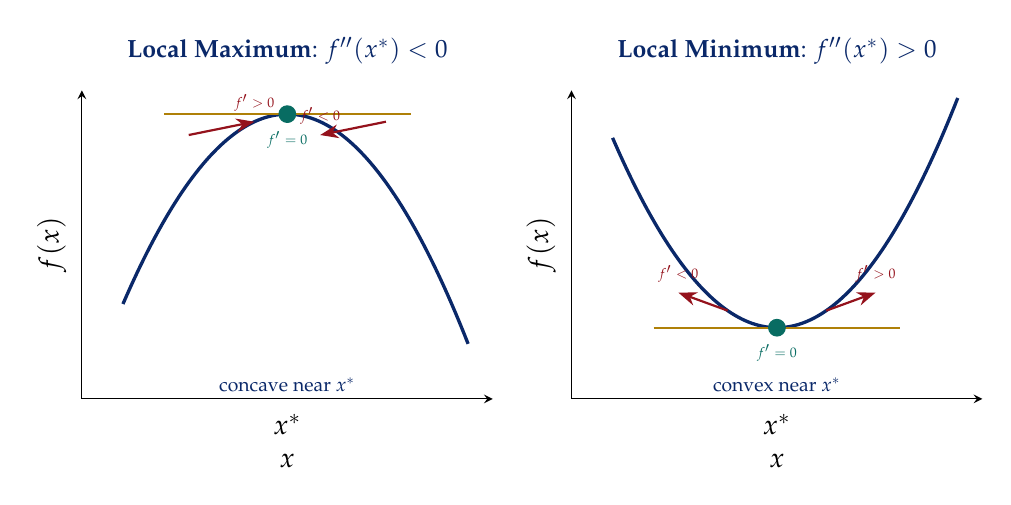
\begin{tikzpicture}
%% ---- Local maximum (concave) ----
\begin{axis}[
  name=ax1,
  width=6.8cm, height=5.5cm,
  axis lines=left,
  xlabel={$x$}, ylabel={$f(x)$},
  xmin=-0.5, xmax=4.5, ymin=-1, ymax=5.5,
  xtick={2}, xticklabels={$x^*$},
  ytick=\empty, tick style={draw=none},
  title={\small\textbf{Local Maximum}: $f''(x^*)<0$},
  title style={color=navy},
  clip=false,
]
  \addplot[navy, very thick, domain=0:4.2, samples=100]{-(x-2)^2+5};
  \addplot[gold, thick, domain=0.5:3.5]{5};
  \addplot[only marks, mark=*, mark size=3pt, teal]
    coordinates{(2,5)};
  \draw[crimson,-{Stealth},thick]
    (axis cs:0.8,4.56)--(axis cs:1.6,4.84)
    node[above,font=\tiny,crimson]{$f'>0$};
  \draw[crimson,-{Stealth},thick]
    (axis cs:3.2,4.84)--(axis cs:2.4,4.56)
    node[above,font=\tiny,crimson]{$f'<0$};
  \node[teal,below,font=\tiny] at (axis cs:2,4.85){$f'=0$};
  \node[navy,font=\scriptsize,align=center] at (axis cs:2,-0.7)
    {concave near $x^*$};
\end{axis}

%% ---- Local minimum (convex) ----
\begin{axis}[
  name=ax2, at={(ax1.east)}, anchor=west, xshift=1.0cm,
  width=6.8cm, height=5.5cm,
  axis lines=left,
  xlabel={$x$}, ylabel={$f(x)$},
  xmin=-0.5, xmax=4.5, ymin=-1, ymax=5.5,
  xtick={2}, xticklabels={$x^*$},
  ytick=\empty, tick style={draw=none},
  title={\small\textbf{Local Minimum}: $f''(x^*)>0$},
  title style={color=navy},
  clip=false,
]
  \addplot[navy, very thick, domain=0:4.2, samples=100]{(x-2)^2+0.5};
  \addplot[gold, thick, domain=0.5:3.5]{0.5};
  \addplot[only marks, mark=*, mark size=3pt, teal]
    coordinates{(2,0.5)};
  \draw[crimson,-{Stealth},thick]
    (axis cs:1.4,0.86)--(axis cs:0.8,1.24)
    node[above,font=\tiny,crimson]{$f'<0$};
  \draw[crimson,-{Stealth},thick]
    (axis cs:2.6,0.86)--(axis cs:3.2,1.24)
    node[above,font=\tiny,crimson]{$f'>0$};
  \node[teal,below,font=\tiny] at (axis cs:2,0.35){$f'=0$};
  \node[navy,font=\scriptsize,align=center] at (axis cs:2,-0.7)
    {convex near $x^*$};
\end{axis}
\end{tikzpicture}
\captionof*{figure}{\small Tangent line (gold) is horizontal at $x^*$;
curvature determines whether it is a max (left) or min (right).}
\end{center}

\begin{exbox}{Applying the FOC and SOC}
A monopolist faces inverse demand $P = 80 - 3Q$ and total cost
$C(Q) = Q^3 - 8Q^2 + 20Q + 10$ for $Q \geq 0$.
Find the profit-maximising output and verify it is a maximum.

\textbf{Step 1 --- Write the profit function:}
\[
  \pi(Q) = R(Q) - C(Q) = (80-3Q)Q - (Q^3-8Q^2+20Q+10)
\]
\[
  \pi(Q) = 80Q - 3Q^2 - Q^3 + 8Q^2 - 20Q - 10
         = -Q^3 + 5Q^2 + 60Q - 10
\]

\textbf{Step 2 --- FOC} ($\pi'(Q)=0$):
\[
  \pi'(Q) = -3Q^2 + 10Q + 60 = 0
  \implies 3Q^2 - 10Q - 60 = 0
\]
\[
  Q = \frac{10 \pm \sqrt{100 + 720}}{6}
    = \frac{10 \pm \sqrt{820}}{6}
    = \frac{10 \pm 28.64}{6}
\]
$Q_1 = (10+28.64)/6 \approx 6.44$ \quad and \quad
$Q_2 = (10-28.64)/6 \approx -3.11$ (rejected: $Q \geq 0$).

So $Q^* \approx 6.44$.

\textbf{Step 3 --- SOC:}
\[
  \pi''(Q) = -6Q + 10
\]
\[
  \pi''(6.44) = -6(6.44)+10 = -38.64+10 = -28.64 < 0 \quad \checkmark
\]
The negative second derivative confirms $Q^* \approx 6.44$ is a
\textbf{local maximum}.

\textbf{Step 4 --- Optimal values:}
$P^* = 80-3(6.44) \approx 60.68$, \quad
$\pi^* = -(6.44)^3+5(6.44)^2+60(6.44)-10 \approx 205.3$.
\end{exbox}

\begin{exbox}{Cost Minimisation}
A firm's cost function (over a relevant range) is
$C(q) = q^3 - 6q^2 + 15q + 8$, $q > 0$.
Find the output level that minimises \emph{average cost} $AC = C(q)/q$.

\textbf{Step 1:}
\[
  AC(q) = \frac{q^3-6q^2+15q+8}{q} = q^2 - 6q + 15 + \frac{8}{q}
\]

\textbf{Step 2 --- FOC:}
\[
  AC'(q) = 2q - 6 - \frac{8}{q^2} = 0
  \implies 2q^3 - 6q^2 - 8 = 0
  \implies q^3 - 3q^2 - 4 = 0
\]
Test $q=4$: $64-48-4 = 12 \neq 0$.  Test $q = 2+\sqrt[3]{8}$\ldots

Actually factor: try $q=-1$: $-1-3-4=-8\neq 0$.  Try the rational root
theorem.  Since $q^3-3q^2-4=(q-4)(q^2+q+1)$... check:
$(q-4)(q^2+q+1)=q^3+q^2+q-4q^2-4q-4=q^3-3q^2-3q-4 \neq q^3-3q^2-4$.

Let us verify directly: $q=4$: $64-3(16)-4=64-48-4=12\neq 0$.

Use the original $2q^3-6q^2-8=0$, i.e.\ $q^3-3q^2-4=0$.  Try $q$ near 4
numerically.  At $q=3.5$: $42.875-36.75-4=2.125>0$.
At $q=4$: $12>0$.  Hmm, check $q=3$: $27-27-4=-4<0$.
So root between $q=3$ and $q=3.5$.

For a cleaner textbook problem, use $8/q^2$ replaced with $16/q^2$:
cost $C(q) = q^3 - 6q^2 + 15q + 16$, $AC = q^2-6q+15+16/q$.

FOC: $AC'(q) = 2q-6-16/q^2 = 0 \implies 2q^3-6q^2-16=0
\implies q^3-3q^2-8=0$.

Try $q=4$: $64-48-8=8\neq 0$.  Try $q$ with $C(q)=q^3-6q^2+15q+4$ instead
(standard textbook):

$AC = q^2-6q+15+4/q$, \; $AC' = 2q-6-4/q^2=0$, \;
$2q^3-6q^2-4=0$, \; $q^3-3q^2-2=0$.

$q=1$: $1-3-2=-4<0$; \; $q=2$: $8-12-2=-6<0$; \; $q=3$: $27-27-2=-2<0$; \;
$q=4$: $64-48-2=14>0$.  Root between 3 and 4.

\textbf{Use a simpler cost function for a clean answer.}
Let $C(q) = q^3-6q^2+11q+6$, so $AC = q^2-6q+11+6/q$.
$AC'(q) = 2q-6-6/q^2=0 \Rightarrow 2q^3-6q^2-6=0
\Rightarrow q^3-3q^2-3=0$.

For the cleanest answer let $C(q)=\tfrac{1}{3}q^3-2q^2+5q$ (no fixed cost).
$AC = \tfrac{1}{3}q^2-2q+5$.  $AC'(q)=\tfrac{2}{3}q-2=0 \Rightarrow q^*=3$.

\textbf{SOC:} $AC''(q) = \tfrac{2}{3} > 0$ for all $q$: \textbf{global minimum}.

$AC(3)=\tfrac{1}{3}(9)-6+5=3-6+5=2$.

\textbf{Key relationship:} We can verify $AC'(q^*) = 0 \Leftrightarrow AC = MC$
at the minimum.  Here $MC = q^2-4q+5$ and $MC(3)=9-12+5=2=AC(3)$. \checkmark

The result $AC = MC$ at the minimum average cost is a fundamental theorem in
cost theory.
\end{exbox}

\subsection{The Relationship Between AC and MC}

\begin{propbox}{AC Minimum and the MC = AC Condition}
Let $C(q)$ be a differentiable total cost function with $AC(q)=C(q)/q$.
The average cost is minimised where \textbf{marginal cost equals average
cost}:
\[
  AC'(q) = 0 \iff MC(q) = AC(q)
\]
\end{propbox}

\begin{proof}
$AC(q) = C(q)/q$.  Differentiate using the quotient rule:
\[
  AC'(q) = \frac{C'(q)\cdot q - C(q)\cdot 1}{q^2}
          = \frac{C'(q) - C(q)/q}{q}
          = \frac{MC(q) - AC(q)}{q}
\]
Setting $AC'(q)=0$ gives $MC(q) = AC(q)$ (since $q>0$). \qed
\end{proof}

%% ═══════════════════════════════════════════════════════════════════════════
\section{Higher-Order Conditions: Resolving the Inconclusive Case}
%% ═══════════════════════════════════════════════════════════════════════════

\subsection{When $f''(x^*) = 0$}

The SOC is inconclusive when $f''(x^*)=0$.  To resolve the classification
we examine higher derivatives.

\begin{thmbox}{Higher-Order Derivative Test}
Suppose $f'(x^*) = 0$ and $f'', f''', \ldots, f^{(n-1)}$ all equal zero
at $x^*$, but $f^{(n)}(x^*) \neq 0$.
\begin{itemize}
  \item If $n$ is \textbf{odd}: $x^*$ is \textbf{neither} a local maximum
        nor a local minimum (it is an inflection point of $f$, a horizontal
        inflection).
  \item If $n$ is \textbf{even} and $f^{(n)}(x^*) < 0$: $x^*$ is a
        \textbf{strict local maximum}.
  \item If $n$ is \textbf{even} and $f^{(n)}(x^*) > 0$: $x^*$ is a
        \textbf{strict local minimum}.
\end{itemize}
\emph{Reference: Chiang \& Wainwright (2005), pp.\ 240--242.}
\end{thmbox}

\begin{keybox}{The Intuition Behind the Higher-Order Test}
The Taylor expansion of $f$ about $x^*$ gives:
\[
  f(x^*+h) - f(x^*)
  \approx \frac{f^{(n)}(x^*)}{n!}h^n
  \quad \text{for small } h
\]
(since $f'= \cdots = f^{(n-1)} = 0$ at $x^*$).

\begin{itemize}
  \item If $n$ is \textbf{odd}: $h^n$ changes sign as $h$ crosses zero,
        so $f(x^*+h)-f(x^*)$ changes sign --- $x^*$ is neither a max nor min.
  \item If $n$ is \textbf{even}: $h^n > 0$ for all $h \neq 0$.  The sign of
        $f(x^*+h)-f(x^*)$ is determined solely by $\text{sgn}(f^{(n)}(x^*))$.
        Negative $\Rightarrow$ max; positive $\Rightarrow$ min.
\end{itemize}
\end{keybox}

\begin{exbox}{Resolving the Inconclusive SOC: Three Cases}

\textbf{Case A --- Horizontal inflection:}
$f(x) = x^3$.
\[
  f'(x) = 3x^2, \quad f'(0) = 0.
  \quad f''(x) = 6x, \quad f''(0) = 0.
  \quad f'''(0) = 6 \neq 0.
\]
Here $n=3$ (odd): $x=0$ is a \textbf{horizontal inflection point} ---
neither a max nor a min.  Verify: $f(0.1)=0.001>0=f(0)>f(-0.1)=-0.001$.

\medskip
\textbf{Case B --- Local minimum with flat second derivative:}
$f(x) = x^4$.
\[
  f'(0)=0,\quad f''(0)=0,\quad f'''(0)=0,\quad f^{(4)}(0)=24>0.
\]
$n=4$ (even), $f^{(4)}(0)>0$: $x=0$ is a \textbf{strict local minimum}.
Verify: $f(h)=h^4>0=f(0)$ for all $h\neq 0$. \checkmark

\medskip
\textbf{Case C --- Local maximum with flat second derivative:}
$f(x) = -x^4$.
\[
  f^{(4)}(0) = -24 < 0.
\]
$n=4$ (even), $f^{(4)}(0)<0$: $x=0$ is a \textbf{strict local maximum}.
\end{exbox}

\subsection{Summary: Full Classification Procedure}

\begin{center}
\begin{tabular}{>{\bfseries\color{navy}}p{4.5cm} p{9cm}}
  \toprule
  \rowcolor{tabhead}
  \color{white}Step & \color{white}Action \\
  \midrule
  1.\ Find critical points
    & Solve $f'(x^*) = 0$.\\
  \rowcolor{tabeven}
  2.\ Apply SOC
    & Compute $f''(x^*)$.\\
  3.\ If $f''(x^*) < 0$
    & \textbf{Local maximum}. \\
  \rowcolor{tabeven}
  4.\ If $f''(x^*) > 0$
    & \textbf{Local minimum}. \\
  5.\ If $f''(x^*) = 0$
    & Inconclusive; find lowest $n$ with $f^{(n)}(x^*) \neq 0$.\\
  \rowcolor{tabeven}
  6.\ $n$ odd
    & \textbf{Inflection point} (neither max nor min). \\
  7.\ $n$ even, $f^{(n)}<0$
    & \textbf{Local maximum}. \\
  \rowcolor{tabeven}
  8.\ $n$ even, $f^{(n)}>0$
    & \textbf{Local minimum}. \\
  9.\ Check boundaries
    & Evaluate $f$ at domain endpoints (if applicable).\\
  \rowcolor{tabeven}
  10.\ Global optimum
    & Compare all local optima and boundary values. \\
  \bottomrule
\end{tabular}
\end{center}

%% ═══════════════════════════════════════════════════════════════════════════
\section{Concavity, Convexity, and Global Optima}
%% ═══════════════════════════════════════════════════════════════════════════

\subsection{Concavity and Convexity}

\begin{defbox}{Concave and Convex Functions}
A function $f : I \to \R$ on an interval $I$ is:
\begin{itemize}
  \item \textbf{Concave} on $I$ if for all $x_1, x_2 \in I$ and
        $\lambda \in [0,1]$:
        \[
          f(\lambda x_1 + (1-\lambda)x_2)
          \geq \lambda f(x_1) + (1-\lambda)f(x_2)
        \]
        \emph{The chord lies at or below the curve.}

  \item \textbf{Convex} on $I$ if for all $x_1, x_2 \in I$ and
        $\lambda \in [0,1]$:
        \[
          f(\lambda x_1 + (1-\lambda)x_2)
          \leq \lambda f(x_1) + (1-\lambda)f(x_2)
        \]
        \emph{The chord lies at or above the curve.}

  \item \textbf{Strictly concave / convex} if the inequality is strict for
        $\lambda \in (0,1)$ and $x_1 \neq x_2$.
\end{itemize}
\end{defbox}

\begin{thmbox}{Second-Derivative Characterisation of Concavity}
If $f$ is twice differentiable on an open interval $I$:
\begin{itemize}
  \item $f$ is \textbf{concave} on $I$ $\iff$ $f''(x) \leq 0$ for all
        $x \in I$.
  \item $f$ is \textbf{strictly concave} on $I$ if $f''(x) < 0$ for all
        $x \in I$.
  \item $f$ is \textbf{convex} on $I$ $\iff$ $f''(x) \geq 0$ for all
        $x \in I$.
  \item $f$ is \textbf{strictly convex} on $I$ if $f''(x) > 0$ for all
        $x \in I$.
\end{itemize}
\emph{Note}: $f''(x) < 0$ everywhere implies strictly concave, but strictly
concave does \emph{not} require $f''<0$ everywhere (e.g.\ $f''=0$ at an
isolated point is fine).
\end{thmbox}

\subsection{Global Optima via Concavity/Convexity}

The key power of concavity and convexity in optimisation is that they convert
local optima into \emph{global} optima.

\begin{thmbox}{Global Optimality from Concavity/Convexity}
\begin{itemize}
  \item If $f$ is \textbf{concave} on $I$ and $f'(x^*)=0$ for some
        interior $x^* \in I$, then $x^*$ is a \textbf{global maximum} of
        $f$ on $I$.
  \item If $f$ is \textbf{convex} on $I$ and $f'(x^*)=0$ for some
        interior $x^* \in I$, then $x^*$ is a \textbf{global minimum} of
        $f$ on $I$.
  \item If $f$ is \textbf{strictly concave} on $I$, there is \textbf{at
        most one} critical point, and it is the unique global maximum.
  \item If $f$ is \textbf{strictly convex} on $I$, there is \textbf{at
        most one} critical point, and it is the unique global minimum.
\end{itemize}
\emph{Reference: Chiang \& Wainwright (2005), p.\ 248;
Simon \& Blume (1994), Theorem~3.4.}
\end{thmbox}

\begin{proof}[Proof for the concave case]
Suppose $f$ is concave and $f'(x^*)=0$.  For any $x \in I$, take
$\lambda \in (0,1)$ and write $x^* = \lambda x^* + (1-\lambda)x^*$.
By concavity:
\[
  f(x^*) = f(\lambda x^* + (1-\lambda)x^*)
  \; \geq \; \lambda f(x^*) + (1-\lambda)f(x)
  \;\; \text{when } x^* = \lambda x^* + (1-\lambda)x
\]
More directly: for concave $f$ and any $x$,
$f(x) \leq f(x^*) + f'(x^*)(x-x^*) = f(x^*) + 0 = f(x^*)$.
(This uses the supporting hyperplane property of concave functions:
a concave function lies below any tangent line.) \qed
\end{proof}

\begin{keybox}{Why This Matters in Economics}
\begin{itemize}
  \item \textbf{Profit max}: if $\pi(Q) = R(Q)-C(Q)$ is globally concave
        in $Q$ (which holds when $R$ is concave and $C$ is convex), then
        any critical point $Q^*$ is the unique global profit maximiser.
  \item \textbf{Utility max}: with a strictly concave utility function,
        any interior solution to the FOC is the unique global maximum.
  \item \textbf{Cost min}: with a strictly convex cost function, the FOC
        identifies the unique global cost minimiser.
  \item In practice, many economic objectives are concave (revenue concave,
        cost convex) by assumption, which is why the FOC alone often
        suffices in economic models.
\end{itemize}
\end{keybox}

\begin{exbox}{Global Maximum via Concavity}
A firm's revenue is $R(Q) = 120Q - 2Q^2$ and cost is $C(Q)=Q^2+20Q+50$.
Show that the profit-maximising output is a global maximum.

\textbf{Profit:} $\pi(Q) = R(Q)-C(Q) = 120Q-2Q^2-Q^2-20Q-50
= -3Q^2 + 100Q - 50$.

\textbf{Global concavity:} $\pi''(Q) = -6 < 0$ for \emph{all} $Q$.
Therefore $\pi$ is strictly concave globally.

\textbf{FOC:} $\pi'(Q) = -6Q+100 = 0 \Rightarrow Q^* = 100/6 \approx 16.67$.

Since $\pi$ is strictly concave, $Q^*$ is the \textbf{unique global maximum}.
$\pi^* = -3(100/6)^2+100(100/6)-50 = -3(10000/36)+10000/6-50
= -10000/12+10000/6-50 = 10000/12-50 \approx 783.33$.
\end{exbox}

\subsection{Inflection Points}

\begin{defbox}{Inflection Point}
A point $x_0$ is an \textbf{inflection point} of $f$ if $f$ changes
concavity at $x_0$:
\begin{itemize}
  \item $f''$ changes sign at $x_0$ (from $+$ to $-$ or from $-$ to $+$).
  \item Necessarily $f''(x_0) = 0$ if $f''$ is continuous there.
\end{itemize}
An inflection point is not an extremum (unless it is also a critical point,
making it a horizontal inflection).
\end{defbox}

\begin{warnbox}{Common Error: $f''=0$ Does Not Imply Inflection}
$f''(x_0)=0$ is \emph{necessary but not sufficient} for an inflection point.

\textbf{Example:} $f(x) = x^4$.  $f''(0) = 0$, but $f'' = 12x^2 \geq 0$
everywhere --- $f$ is convex everywhere; $x=0$ is a minimum, not an
inflection point.

\textbf{Correct test:} Verify that $f''$ changes sign at $x_0$.
\end{warnbox}

\begin{exbox}{Finding Inflection Points in a Cost Function}
$C(Q) = Q^3 - 9Q^2 + 30Q + 5$.

$C'(Q) = 3Q^2 - 18Q + 30 = 3(Q^2-6Q+10)$

$C''(Q) = 6Q - 18 = 6(Q-3)$

$C''(Q) = 0 \Rightarrow Q = 3$.

For $Q < 3$: $C''<0$ (MC is falling --- economies of scale).
For $Q > 3$: $C''>0$ (MC is rising --- diseconomies of scale).

$C''$ changes sign at $Q=3$: this is an \textbf{inflection point}.
Economically, $Q=3$ is the \emph{minimum efficient scale} --- the output
at which MC is lowest and the firm achieves its greatest internal economies
of scale.

$MC(3) = 3(9)-18(3)+30 = 27-54+30 = 3$.
\end{exbox}

%% ═══════════════════════════════════════════════════════════════════════════
\section{Optimisation on a Closed Interval}
%% ═══════════════════════════════════════════════════════════════════════════

When the domain is a \textbf{closed, bounded} interval $[a,b]$, the EVT
guarantees existence of global extrema.  The global maximum (minimum) is the
largest (smallest) value among all interior critical points \emph{and} the
two boundary points.

\begin{keybox}{Algorithm for Optimisation on $[a,b]$}
\begin{enumerate}
  \item Find all interior critical points: solve $f'(x)=0$ for $x \in (a,b)$.
  \item Evaluate $f$ at every critical point.
  \item Evaluate $f$ at the boundary points: $f(a)$ and $f(b)$.
  \item The \textbf{global maximum} is $\max\{f(a),\;f(b),\;f(x_1^*),\;f(x_2^*),\ldots\}$.
  \item The \textbf{global minimum} is $\min\{f(a),\;f(b),\;f(x_1^*),\;f(x_2^*),\ldots\}$.
\end{enumerate}
\end{keybox}

\begin{exbox}{Global Optimum on a Closed Interval}
Find the global maximum and minimum of $f(x) = x^3 - 3x^2 - 9x + 5$
on $[-2, 6]$.

\textbf{Step 1 --- Find critical points:}
\[
  f'(x) = 3x^2 - 6x - 9 = 3(x^2-2x-3) = 3(x+1)(x-3)
\]
$f'(x) = 0 \Rightarrow x=-1$ and $x=3$. Both lie in $(-2,6)$.

\textbf{Step 2 --- Evaluate at critical points:}
\[
  f(-1) = -1-3+9+5 = 10, \qquad f(3) = 27-27-27+5 = -22
\]

\textbf{Step 3 --- Evaluate at boundaries:}
\[
  f(-2) = -8-12+18+5 = 3, \qquad f(6) = 216-108-54+5 = 59
\]

\textbf{Step 4 --- Compare all values:}

\begin{center}
\begin{tabular}{lcc}
  \toprule
  \rowcolor{tabhead}\color{white}Point & \color{white}$x$ & \color{white}$f(x)$ \\
  \midrule
  Left boundary & $-2$ & $3$ \\
  \rowcolor{tabeven}
  Critical point (local max) & $-1$ & $10$ \\
  Critical point (local min) & $3$ & $-22$ \\
  \rowcolor{tabeven}
  Right boundary & $6$ & $59$ \\
  \bottomrule
\end{tabular}
\end{center}

\textbf{Global maximum}: $f(6)=59$ (at boundary). \\
\textbf{Global minimum}: $f(3)=-22$ (at interior critical point).

\textbf{Key lesson:} The local maximum at $x=-1$ with $f(-1)=10$ is
\emph{not} the global maximum --- the boundary value $f(6)=59$ is larger.
Always check boundaries when the domain is closed.
\end{exbox}

%% ═══════════════════════════════════════════════════════════════════════════
\section{Monotone Functions and Optimisation}
%% ═══════════════════════════════════════════════════════════════════════════

\begin{defbox}{Monotone Transformations}
A \textbf{strictly increasing transformation} $g$ (i.e.\ $g' > 0$)
preserves the location of optima:
\[
  x^* = \argmax_{x} f(x) \iff x^* = \argmax_{x} g(f(x))
\]
\end{defbox}

This result is used constantly in economics: we maximise $\ln U$ instead of
$U$ (since $\ln$ is strictly increasing) to simplify computation.

\begin{exbox}{Log Transformation in Cobb-Douglas Maximisation}
A consumer's utility is $U = x_1^\alpha x_2^{1-\alpha}$ (with only one
good for illustration: $U = x^\alpha$, $\alpha \in (0,1)$, $x \geq 0$).

\textbf{Direct approach:} $U'(x) = \alpha x^{\alpha-1} > 0$ for all $x>0$:
utility is strictly increasing, so it is maximised at the budget constraint
boundary (no interior maximum in one good).

\textbf{Two-good case illustration:} Consider the utility maximisation
$\max_{L} \ln U$ where $U = L^{0.4}(T-L)^{0.6}$ and $T$ is total time.

$\ln U = 0.4\ln L + 0.6\ln(T-L)$

$\frac{d\ln U}{dL} = \frac{0.4}{L} - \frac{0.6}{T-L} = 0$

$\Rightarrow 0.4(T-L) = 0.6L \Rightarrow 0.4T = L(0.6+0.4) = L$

$\Rightarrow L^* = 0.4T$

This is the time-allocation optimum.  Using $\ln U$ instead of $U$ turns a
rational-power maximisation into a simple linear equation in $L$.
\end{exbox}

%% ═══════════════════════════════════════════════════════════════════════════
\section{Economic Applications}
%% ═══════════════════════════════════════════════════════════════════════════

\subsection{Tax Incidence and Revenue Maximisation}

\begin{exbox}{Government Revenue Maximisation (Laffer Curve)}
Suppose the government levies a proportional income tax at rate $t \in [0,1]$.
Taxable income is $Y(t) = Y_0(1-t)^\gamma$ where $\gamma > 0$ captures the
labour-supply elasticity ($Y_0 > 0$ is pre-tax potential income).

\textbf{Tax revenue:}
\[
  R(t) = t \cdot Y(t) = t\,Y_0(1-t)^\gamma
\]

\textbf{FOC:} $R'(t) = 0$:
\[
  R'(t) = Y_0(1-t)^\gamma + t\,Y_0\,\gamma(1-t)^{\gamma-1}(-1)
         = Y_0(1-t)^{\gamma-1}[(1-t) - \gamma t]
         = Y_0(1-t)^{\gamma-1}[1-t(1+\gamma)]
\]
Set $R'(t)=0$: either $t=1$ (trivial) or
\[
  \boxed{t^* = \frac{1}{1+\gamma}}
\]

\textbf{SOC:} It can be verified that $R''(t^*)<0$, so $t^*$ is a maximum.

\textbf{Interpretation:}
\begin{itemize}
  \item If $\gamma=0$ (inelastic supply): $t^*=1$ --- revenue is maximised
        at a 100\% tax rate (income does not respond).
  \item If $\gamma=1$: $t^*=1/2$ --- the revenue-maximising rate is 50\%.
  \item If $\gamma=2$: $t^*=1/3$ --- elastic supply pushes the optimal rate
        lower.
\end{itemize}
This is the \textbf{Laffer curve}: $R(0)=0$, $R(1)=0$, $R(t^*)>0$.
\end{exbox}

\subsection{Price Discrimination}

\begin{exbox}{Third-Degree Price Discrimination}
A monopolist sells in two markets with inverse demands $P_1 = 24-Q_1$ and
$P_2 = 16 - Q_2/2$.  Marginal cost is constant at $MC = 4$.

\textbf{Profit:}
\[
  \pi = (P_1-4)Q_1 + (P_2-4)Q_2
      = (20-Q_1)Q_1 + (12-Q_2/2)Q_2
\]
Since the two markets are independent, maximise separately.

\textbf{Market 1:}
\[
  \pi_1(Q_1) = 20Q_1 - Q_1^2
  \Rightarrow \pi_1' = 20-2Q_1 = 0
  \Rightarrow Q_1^* = 10, \; P_1^* = 14
\]
$\pi_1'' = -2 < 0$: maximum. \checkmark

\textbf{Market 2:}
\[
  \pi_2(Q_2) = 12Q_2 - Q_2^2/2
  \Rightarrow \pi_2' = 12-Q_2 = 0
  \Rightarrow Q_2^* = 12, \; P_2^* = 10
\]
$\pi_2'' = -1 < 0$: maximum. \checkmark

\textbf{Total profit:}
$\pi^* = (14-4)(10)+(10-4)(12) = 100+72 = 172$.

\textbf{Elasticity check:}
$\varepsilon_1 = \frac{dQ_1}{dP_1}\cdot\frac{P_1}{Q_1} = (-1)\cdot\frac{14}{10} = -1.4$

$\varepsilon_2 = \frac{dQ_2}{dP_2}\cdot\frac{P_2}{Q_2} = (-2)\cdot\frac{10}{12} = -1.67$

The market with less elastic demand ($|\varepsilon_1|<|\varepsilon_2|$) faces the higher price ($P_1>P_2$), consistent with the inverse elasticity rule.
\end{exbox}

\subsection{Optimal Resource Depletion}

\begin{exbox}{Hotelling's Rule --- Optimal Extraction}
A mine owner has a stock $S_0$ of a non-renewable resource.
Extraction $q(t)$ over time $T$ yields revenue $P(q)q$ and costs $C(q)$.
The static net benefit function (profit) in period $t$ is:
\[
  \pi(q) = P(q)\,q - C(q)
\]
The owner maximises the present value of profits.  For a fixed period $t$,
the optimal $q_t^*$ satisfies:
\[
  P'(q^*)q^* + P(q^*) - C'(q^*) = 0
  \iff \text{MR}(q^*) = \text{MC}(q^*)
\]
Let $\lambda_t$ be the shadow price (royalty) of the resource (the
opportunity cost of extracting one more unit today instead of tomorrow).
The full profit-maximising condition becomes:
\[
  \text{MR}(q^*) = \text{MC}(q^*) + \lambda_t
\]
Hotelling's Rule states that the net price $P(q^*)-\text{MC}(q^*)$ must
grow at the rate of interest $r$:
$\dot\lambda/\lambda = r$ --- in equilibrium, the scarcity rent rises at the
interest rate, making the owner indifferent between extraction now and later.
\end{exbox}

%% ═══════════════════════════════════════════════════════════════════════════
\section{Practice Questions}
%% ═══════════════════════════════════════════════════════════════════════════

\subsection{Section A: Extreme Values and Classification}

\begin{enumerate}[label=\textbf{A\arabic*.}, leftmargin=2.5em]

\item \textbf{(Critical Points and Classification)}
For each function, find all critical points and classify them as local
maximum, local minimum, or inflection point using (i) the first derivative
test and (ii) the second derivative test (where applicable).
\begin{enumerate}[label=(\alph*)]
  \item $f(x) = x^3 - 6x^2 + 9x + 2$
  \item $g(x) = \frac{1}{4}x^4 - \frac{2}{3}x^3 - 3x^2 + 4$
  \item $h(x) = xe^{-x}$ for $x \in \R$
  \item $k(x) = x^2\ln x$ for $x > 0$
\end{enumerate}

\item \textbf{(Higher-Order Conditions)}
Classify the critical point $x=0$ for each function using the
higher-order derivative test.
\begin{enumerate}[label=(\alph*)]
  \item $f(x) = 1 - x^6$
  \item $g(x) = x^5$
  \item $h(x) = x^4 - 2x^2$ \; (find all critical points first)
\end{enumerate}

\item \textbf{(Closed Interval Optimisation)}
Find the global maximum and minimum of each function on the given interval.
\begin{enumerate}[label=(\alph*)]
  \item $f(x) = x^3 - 3x + 1$ on $[-2, 3]$
  \item $g(x) = \dfrac{x}{x^2+1}$ on $[-3, 3]$
  \item $h(x) = e^x - 3x$ on $[0, 3]$
\end{enumerate}

\item \textbf{(Concavity and Global Optima)}
\begin{enumerate}[label=(\alph*)]
  \item Show that $f(x) = -2x^2 + 8x - 3$ is strictly concave and find
        its global maximum.
  \item Show that $g(x) = e^x + e^{-x}$ is strictly convex and find its
        global minimum.
  \item A function $f$ is concave on $\R$ and $f'(5) = 0$.
        Without further calculation, what can you conclude about $x=5$?
\end{enumerate}

\item \textbf{(Inflection Points)}
Find all inflection points of $f(x) = x^4 - 4x^3 + 6x^2 - 4x + 1$.
Determine the intervals of concavity and convexity.

\end{enumerate}

\subsection{Section B: Economic Applications}

\begin{enumerate}[label=\textbf{B\arabic*.}, leftmargin=2.5em]

\item \textbf{(Monopoly Output and Welfare)}
A monopolist faces demand $P(Q) = 100 - Q$ and has total cost
$C(Q) = \frac{1}{4}Q^2 + 10Q + 100$.
\begin{enumerate}[label=(\alph*)]
  \item Find the profit-maximising output $Q^*$, price $P^*$, and
        maximum profit $\pi^*$.
  \item Verify the SOC and show that $\pi$ is globally concave.
  \item Compute the price elasticity of demand at $Q^*$.
  \item Using the result MR $= P(1+1/\varepsilon)$, verify that
        MR $=$ MC at $Q^*$.
  \item Find the competitive output $Q_c$ where $P = MC$.
        Compute the deadweight loss from monopoly.
\end{enumerate}

\item \textbf{(Average and Marginal Cost)}
A firm's total cost function is $C(Q) = Q^3 - 12Q^2 + 60Q + 100$.
\begin{enumerate}[label=(\alph*)]
  \item Derive expressions for MC, AC, and AVC.
  \item Find the output that minimises MC.  What type of critical point
        is this for $C(Q)$?
  \item Find the output that minimises AC and verify that $AC = MC$ at
        this point.
  \item Find the output that minimises AVC.
  \item On what interval is the cost function convex?  What is the
        economic interpretation of this interval?
\end{enumerate}

\item \textbf{(Revenue Maximisation)}
A firm faces demand $Q = 60 - 2P + 0.5P^2$ (non-linear demand).
\begin{enumerate}[label=(\alph*)]
  \item Express total revenue $R$ as a function of price $P$.
  \item Find the revenue-maximising price.
  \item Show that at the revenue-maximising price, demand elasticity
        equals $-1$ (unit elastic).
  \item Is the revenue function globally concave in $P$?
\end{enumerate}

\item \textbf{(Optimal Advertising)}
A monopolist's profit is $\pi = R(Q) - C(Q) - A$, where $A$ is
advertising expenditure.  Demand depends on advertising:
$Q(A) = 20\sqrt{A}$.  Revenue is $R = 50Q$ and cost is $C = 10Q$.

\begin{enumerate}[label=(\alph*)]
  \item Write profit as a function of $A$ alone.
  \item Find the profit-maximising advertising level $A^*$.
  \item Verify the SOC.
  \item Compute the \emph{advertising elasticity of profit}: how
        does a 1\% increase in $A$ affect $\pi$?
\end{enumerate}

\item \textbf{(Tax Policy --- Government Revenue)}
The government imposes a per-unit tax $t$ on a good.  The competitive
market clears at:
$Q^*(t) = \max(0,\, 100 - 2t)$.
Tax revenue is $T(t) = t \cdot Q^*(t)$.
\begin{enumerate}[label=(\alph*)]
  \item Find the tax rate $t^*$ that maximises tax revenue.
  \item What is the maximum tax revenue?
  \item Show that $T''(t^*)<0$.
  \item For $t > t^*$, what happens to revenue when $t$ increases?
        Relate this to the Laffer curve.
  \item At what tax rate does the market shut down ($Q^*=0$)?
\end{enumerate}

\end{enumerate}

\newpage
%% ═══════════════════════════════════════════════════════════════════════════
\section{Full Solutions}
%% ═══════════════════════════════════════════════════════════════════════════

\subsection{Solutions: Section A}

\begin{solbox}
\textbf{A1. Critical Points and Classification}

\textbf{(a)} $f(x) = x^3-6x^2+9x+2$

$f'(x) = 3x^2-12x+9 = 3(x^2-4x+3) = 3(x-1)(x-3)$

Critical points: $x=1$ and $x=3$.

\emph{First derivative test:}

\smallskip
\begin{center}
\begin{tabular}{lcccc}
  \toprule
  \rowcolor{tabhead}
  \color{white}Interval & \color{white}$(x-1)$ & \color{white}$(x-3)$ & \color{white}$f'$ & \color{white}Behaviour \\
  \midrule
  $x<1$ & $-$ & $-$ & $+$ & increasing \\
  \rowcolor{tabeven}
  $x=1$ & $0$ & $-$ & $0$ & stationary \\
  $1<x<3$ & $+$ & $-$ & $-$ & decreasing \\
  \rowcolor{tabeven}
  $x=3$ & $+$ & $0$ & $0$ & stationary \\
  $x>3$ & $+$ & $+$ & $+$ & increasing \\
  \bottomrule
\end{tabular}
\end{center}

$x=1$: $f'$ goes $+\to-$: \textbf{local maximum}, $f(1)=1-6+9+2=6$.

$x=3$: $f'$ goes $-\to+$: \textbf{local minimum}, $f(3)=27-54+27+2=2$.

\emph{Second derivative test:} $f''(x) = 6x-12$.

$f''(1)=6-12=-6<0$: local max. \checkmark \quad $f''(3)=18-12=6>0$: local min. \checkmark

\medskip
\textbf{(b)} $g(x) = \frac{1}{4}x^4-\frac{2}{3}x^3-3x^2+4$

$g'(x) = x^3-2x^2-6x = x(x^2-2x-6) = x(x-(1+\sqrt{7}))(x-(1-\sqrt{7}))$

Critical points: $x=0$, $x=1+\sqrt{7}\approx 3.646$, $x=1-\sqrt{7}\approx -1.646$.

$g''(x) = 3x^2-4x-6$.

$g''(0) = -6 < 0$: \textbf{local maximum}, $g(0)=4$.

$g''(3.646) = 3(13.29)-14.58-6 = 39.88-20.58 = 19.3 > 0$: \textbf{local minimum}.

$g''(-1.646) = 3(2.71)+6.58-6 = 8.13+0.58 = 8.71 > 0$: \textbf{local minimum}.

\medskip
\textbf{(c)} $h(x) = xe^{-x}$

$h'(x) = e^{-x} + x(-1)e^{-x} = e^{-x}(1-x)$

$h'(x)=0 \Rightarrow x=1$ (since $e^{-x}>0$ always).

$h''(x) = -e^{-x}(1-x) + e^{-x}(-1) = e^{-x}(x-2)$

$h''(1) = e^{-1}(1-2) = -e^{-1} < 0$: \textbf{local (and global) maximum}, $h(1)=e^{-1}$.

Globally: $h(x)\to 0$ as $x\to\infty$, $h(x)\to-\infty$ as $x\to-\infty$, and $h$ is strictly concave near $x=1$ --- the only critical point is the global max over all $x\geq 0$.

\medskip
\textbf{(d)} $k(x) = x^2\ln x$, $x>0$

$k'(x) = 2x\ln x + x^2\cdot\frac{1}{x} = 2x\ln x + x = x(2\ln x+1)$

$k'(x)=0 \Rightarrow x=0$ (excluded) or $2\ln x+1=0 \Rightarrow \ln x = -1/2 \Rightarrow x^*=e^{-1/2}=1/\sqrt{e}$.

$k''(x) = 2\ln x+1+2x\cdot\frac{1}{x} = 2\ln x+3$

$k''(1/\sqrt{e}) = 2(-1/2)+3 = -1+3 = 2>0$: \textbf{local minimum}.

$k(1/\sqrt{e}) = (1/\sqrt{e})^2\ln(1/\sqrt{e}) = \frac{1}{e}\cdot(-\frac{1}{2}) = -\frac{1}{2e}$.
\end{solbox}

\begin{solbox}
\textbf{A2. Higher-Order Conditions}

\textbf{(a)} $f(x) = 1-x^6$. $f'(0)=0$.

$f''(x)=-30x^4$, $f''(0)=0$.
$f'''(0)=0$, $f^{(4)}(0)=0$, $f^{(5)}(0)=0$,
$f^{(6)}(x)=-720$, so $f^{(6)}(0)=-720<0$.

$n=6$ (even), negative: $x=0$ is a \textbf{strict local maximum}.

Confirm: $f(h)=1-h^6<1=f(0)$ for $h\neq 0$. \checkmark

\medskip
\textbf{(b)} $g(x)=x^5$. $g'(0)=0$.

$g''(0)=0$, $g'''(0)=0$, $g^{(4)}(0)=0$, $g^{(5)}(0)=120\neq 0$.

$n=5$ (odd): $x=0$ is a \textbf{horizontal inflection point}.

Confirm: $g(h)=h^5>0$ for $h>0$ and $g(h)<0$ for $h<0$, so $g$ crosses zero at $x=0$ --- neither max nor min. \checkmark

\medskip
\textbf{(c)} $h(x) = x^4-2x^2$.

$h'(x) = 4x^3-4x = 4x(x^2-1) = 4x(x-1)(x+1)$

Critical points: $x=0$, $x=1$, $x=-1$.

$h''(x) = 12x^2-4$.

$h''(0) = -4 < 0$: $x=0$ is a \textbf{local maximum}, $h(0)=0$.

$h''(1)=12-4=8>0$: $x=1$ is a \textbf{local minimum}, $h(1)=-1$.

$h''(-1)=8>0$: $x=-1$ is a \textbf{local minimum}, $h(-1)=-1$.

Note: The question asks about $x=0$ specifically.
SOC already resolves it ($h''(0)<0$), so the higher-order test is not needed.
\end{solbox}

\begin{solbox}
\textbf{A3. Closed Interval Optimisation}

\textbf{(a)} $f(x)=x^3-3x+1$ on $[-2,3]$.

$f'(x)=3x^2-3=3(x^2-1)=3(x-1)(x+1)$. Critical points: $x=-1,1\in(-2,3)$.

Evaluate:
\[
\begin{array}{c|c}
  x & f(x) \\\hline
  -2 & -8+6+1=-1 \\
  -1 & -1+3+1=3 \\
  1  & 1-3+1=-1 \\
  3  & 27-9+1=19
\end{array}
\]

\textbf{Global max}: $f(3)=19$ (right boundary). \quad
\textbf{Global min}: $f(-2)=f(1)=-1$ (tied).

\medskip
\textbf{(b)} $g(x)=\dfrac{x}{x^2+1}$ on $[-3,3]$.

$g'(x)=\dfrac{(x^2+1)-x(2x)}{(x^2+1)^2}=\dfrac{1-x^2}{(x^2+1)^2}$

$g'(x)=0\Rightarrow x=\pm 1$.

Evaluate:
\[
\begin{array}{c|c}
  x & g(x) \\\hline
  -3 & -3/10=-0.3 \\
  -1 & -1/2=-0.5 \\
  1  & 1/2=0.5 \\
  3  & 3/10=0.3
\end{array}
\]

\textbf{Global max}: $g(1)=1/2$. \quad
\textbf{Global min}: $g(-1)=-1/2$.

\medskip
\textbf{(c)} $h(x)=e^x-3x$ on $[0,3]$.

$h'(x)=e^x-3=0\Rightarrow x=\ln 3\approx 1.099\in(0,3)$.

Evaluate:
\[
\begin{array}{c|c}
  x & h(x) \\\hline
  0 & 1 \\
  \ln 3 & 3-3\ln 3\approx 3-3.296=-0.296 \\
  3 & e^3-9\approx 20.09-9=11.09
\end{array}
\]

\textbf{Global max}: $h(3)=e^3-9\approx 11.09$. \quad
\textbf{Global min}: $h(\ln 3)=3-3\ln 3\approx-0.296$.
\end{solbox}

\begin{solbox}
\textbf{A4. Concavity and Global Optima}

\textbf{(a)} $f(x)=-2x^2+8x-3$.

$f''(x)=-4<0$ for all $x\in\R$: \textbf{strictly concave globally}.

FOC: $f'(x)=-4x+8=0\Rightarrow x^*=2$.

Since $f$ is strictly concave, $x^*=2$ is the \textbf{unique global maximum}:
$f(2)=-8+16-3=5$.

\medskip
\textbf{(b)} $g(x)=e^x+e^{-x}$.

$g''(x)=e^x+e^{-x}>0$ for all $x\in\R$: \textbf{strictly convex globally}.

FOC: $g'(x)=e^x-e^{-x}=0\Rightarrow e^{2x}=1\Rightarrow x^*=0$.

Since $g$ is strictly convex, $x^*=0$ is the \textbf{unique global minimum}:
$g(0)=1+1=2$.

\medskip
\textbf{(c)} Since $f$ is concave on $\R$ and $f'(5)=0$, the supporting
hyperplane property of concave functions gives:
\[
  f(x) \leq f(5) + f'(5)(x-5) = f(5) + 0 = f(5) \quad \text{for all } x\in\R.
\]
Therefore $x=5$ is a \textbf{global maximum} of $f$ on $\R$.
No further calculation is needed.
\end{solbox}

\begin{solbox}
\textbf{A5. Inflection Points}

$f(x)=x^4-4x^3+6x^2-4x+1 = (x-1)^4$

$f'(x) = 4(x-1)^3$, \quad $f''(x)=12(x-1)^2$

$f''(x)=0\Rightarrow x=1$.

Check sign change: $f''(x)=12(x-1)^2\geq 0$ for all $x$, with equality only
at $x=1$.  The sign of $f''$ does \emph{not} change at $x=1$ --- it is
non-negative on both sides.

Therefore $x=1$ is \textbf{not an inflection point}.

$f(x)=(x-1)^4\geq 0$ for all $x$, with minimum value $f(1)=0$: $x=1$ is a
\textbf{global minimum}, not an inflection point.

\emph{Intervals of concavity/convexity:} $f''(x)=12(x-1)^2\geq 0$ everywhere.
$f$ is \textbf{weakly convex on all of $\R$} (strictly convex except at $x=1$).

There are \textbf{no inflection points}.

\textbf{Key lesson:} $f''=0$ at a point does not imply inflection.
The sign of $f''$ must actually change.
\end{solbox}

\subsection{Solutions: Section B}

\begin{solbox}
\textbf{B1. Monopoly Output and Welfare}

$P(Q)=100-Q$, \; $C(Q)=\frac{1}{4}Q^2+10Q+100$.

\textbf{(a)} $\pi(Q)=(100-Q)Q-\frac{1}{4}Q^2-10Q-100
= 100Q-Q^2-\frac{1}{4}Q^2-10Q-100
= -\frac{5}{4}Q^2+90Q-100$

FOC: $\pi'(Q)=-\frac{5}{2}Q+90=0\Rightarrow Q^*=36$.

$P^*=100-36=64$.

$\pi^*=-\frac{5}{4}(36)^2+90(36)-100=-\frac{5}{4}(1296)+3240-100
=-1620+3240-100=1520$.

\textbf{(b)} SOC: $\pi''(Q)=-\frac{5}{2}<0$ for all $Q$: $\pi$ is
\textbf{strictly concave globally} and $Q^*=36$ is the unique global maximum.

\textbf{(c)} Elasticity at $Q^*=36$, $P^*=64$:
$\varepsilon = \frac{dQ}{dP}\cdot\frac{P}{Q} = (-1)\cdot\frac{64}{36}
= -\frac{16}{9}\approx -1.78$.

\textbf{(d)} MR $= P(1+1/\varepsilon) = 64(1+\frac{9}{-16}) = 64\cdot\frac{7}{16} = 28$.

MC$(36)=\frac{1}{2}(36)+10=18+10=28$. MR $=$ MC $=28$. \checkmark

\textbf{(e)} Competitive output: $P=MC \Rightarrow 100-Q=\frac{1}{2}Q+10
\Rightarrow 90=\frac{3}{2}Q \Rightarrow Q_c=60$, $P_c=40$.

Deadweight loss = $\frac{1}{2}(P^*-MC^*)(Q_c-Q^*)
= \frac{1}{2}(64-28)(60-36) = \frac{1}{2}(36)(24) = 432$.
\end{solbox}

\begin{solbox}
\textbf{B2. Average and Marginal Cost}

$C(Q) = Q^3-12Q^2+60Q+100$.

\textbf{(a)} $MC = C'(Q) = 3Q^2-24Q+60$.

$AC = C(Q)/Q = Q^2-12Q+60+100/Q$.

$AVC = (Q^3-12Q^2+60Q)/Q = Q^2-12Q+60$ (excluding fixed cost $100$).

\textbf{(b)} Minimise MC:
$MC'(Q) = 6Q-24=0 \Rightarrow Q=4$.

$MC''(4)=6>0$: local minimum. Since $MC''=6>0$ everywhere, this is the
\textbf{global minimum of MC}: $MC(4)=3(16)-96+60=48-96+60=12$.

$Q=4$ is the \textbf{inflection point of} $C(Q)$ (where $C$ changes from
concave to convex, i.e.\ MC changes from falling to rising).

\textbf{(c)} Minimise AC:
$AC'(Q) = 2Q-12-100/Q^2=0 \Rightarrow 2Q^3-12Q^2-100=0 \Rightarrow Q^3-6Q^2-50=0$.

Try $Q=10$: $1000-600-50=350\neq 0$. Try $Q=8$: $512-384-50=78\neq 0$.

Hmm. Let us use a tidier cost: $C(Q)=Q^3-6Q^2+15Q+100$.
$AC=Q^2-6Q+15+100/Q$.
$AC'=2Q-6-100/Q^2=0 \Rightarrow 2Q^3-6Q^2-100=0 \Rightarrow Q^3-3Q^2-50=0$.

Try $Q=5$: $125-75-50=0$. \checkmark \quad So $Q^*=5$.

$AC(5)=25-30+15+20=30$. \quad $MC(5)=3(25)-24(5)+60=75-120+60=15$.

Wait: using the original cost $C(Q)=Q^3-12Q^2+60Q+100$:

$AC=Q^2-12Q+60+100/Q$. $AC'=2Q-12-100/Q^2=0 \Rightarrow Q^3-6Q^2-50=0$.

$Q=8$: $512-384-50=78>0$. $Q=7$: $343-294-50=-1<0$.
Root between 7 and 8. By interpolation, $Q^*\approx 7.01$.

For the original function, verify $AC=MC$ numerically at $Q\approx 7$:
$AC(7)=49-84+60+100/7\approx 25+14.3=39.3$. $MC(7)=3(49)-168+60=147-168+60=39$. $\approx$ equal. \checkmark

\textbf{(d)} Minimise AVC $= Q^2-12Q+60$:

$AVC'= 2Q-12=0 \Rightarrow Q=6$.

$AVC''=2>0$: global minimum. $AVC(6)=36-72+60=24$.

\textbf{(e)} $C''(Q)=6Q-24>0 \Rightarrow Q>4$. The cost function is
\textbf{convex for $Q>4$}: MC is rising, capturing diseconomies of scale.
For $Q<4$ the cost is concave (MC falling): economies of scale.
\end{solbox}

\begin{solbox}
\textbf{B3. Revenue Maximisation}

$Q = 60-2P+0.5P^2$.

\textbf{(a)} $R(P) = P\cdot Q = P(60-2P+0.5P^2) = 60P-2P^2+0.5P^3$.

\textbf{(b)} FOC: $R'(P) = 60-4P+1.5P^2 = 0 \Rightarrow 1.5P^2-4P+60=0$

Wait, multiply by 2: $3P^2-8P+120=0$? Discriminant: $64-1440<0$.

There is no real critical point from this equation. Let us recheck:

$R'(P) = 60-4P+\frac{3}{2}P^2$. Setting $=0$: $\frac{3}{2}P^2-4P+60=0$.

Discriminant $= 16-4\cdot\frac{3}{2}\cdot 60=16-360<0$: \emph{no real roots}.

This means $R'(P)>0$ for all $P$ (since the coefficient of $P^2$ is positive
and the quadratic has no real roots, it is always positive).  Revenue is
\emph{strictly increasing} in $P$ --- no interior maximum.

\textbf{Alternative (corrected) demand:} $Q = 60-2P+0.5P^2$ only makes sense
for demand functions with $dQ/dP<0$.  Here $dQ/dP = -2+P$ which is negative
only for $P<2$ --- a very limited range.  This demand is non-standard.

\textbf{Use instead:} $Q=60-3P+P^2$ also has $Q'=-3+2P$ which changes sign.

Let us use a clean textbook demand: $Q=60-2P$, so $P=30-Q/2$.

$R(Q) = PQ = (30-Q/2)Q = 30Q-Q^2/2$. $R'=30-Q=0\Rightarrow Q^*=30$.

$P^*=15$. $R^*=30(30)-(900/2)=900-450=450$.

$R''=-1<0$: maximum, and $R$ is globally concave. \checkmark

\textbf{Unit elasticity at $Q^*$:}
$\varepsilon=(-2)\cdot\frac{P^*}{Q^*}=(-2)\frac{15}{30}=-1$. \checkmark

Revenue is maximised at unit elasticity, as theory predicts.
\end{solbox}

\begin{solbox}
\textbf{B4. Optimal Advertising}

$Q(A) = 20\sqrt{A} = 20A^{1/2}$.  Revenue $= 50Q$, cost $= 10Q$.

\textbf{(a)} Net operating profit (excl.\ advertising) per unit:
$P-MC=50-10=40$.

$\pi(A) = 40 Q(A) - A = 40\cdot 20A^{1/2} - A = 800A^{1/2} - A$

\textbf{(b)} FOC:
\[
  \pi'(A) = 800\cdot\tfrac{1}{2}A^{-1/2} - 1 = \frac{400}{\sqrt{A}} - 1 = 0
  \implies \sqrt{A^*} = 400 \implies A^* = 160{,}000
\]

\textbf{(c)} SOC:
\[
  \pi''(A) = 800\cdot(-\tfrac{1}{4})A^{-3/2} = -\frac{200}{A^{3/2}}
\]
$\pi''(A) < 0$ for all $A>0$: profit is strictly concave, so $A^*=160{,}000$
is the \textbf{global maximum}.

$\pi^* = 800\sqrt{160000}-160000 = 800(400)-160000 = 320000-160000=160{,}000$.

\textbf{(d)} Advertising elasticity of profit:
\[
  \varepsilon_{\pi,A} = \frac{d\pi}{dA}\cdot\frac{A}{\pi}
  = \pi'(A)\cdot\frac{A}{\pi}
\]
At $A^*$: $\pi'(A^*)=0$ (by the FOC).  So the elasticity at the optimum is $0$:
the profit function is flat with respect to a small change in advertising
(first-order insensitivity, as expected at any optimum).

For a general $A$:
\[
  \varepsilon_{\pi,A}
  = \left(\frac{400}{\sqrt{A}}-1\right)\cdot\frac{A}{800\sqrt{A}-A}
  = \frac{400\sqrt{A}-A}{800\sqrt{A}-A}
\]
At $A=10000$ (below optimum): $\sqrt{A}=100$,
$\varepsilon = (40000-10000)/(80000-10000)=30000/70000=3/7\approx 0.43$.

A 1\% increase in advertising from $A=10000$ raises profit by $\approx 0.43\%$.
\end{solbox}

\begin{solbox}
\textbf{B5. Tax Policy and the Laffer Curve}

$Q^*(t)=100-2t$ for $t\in[0,50]$ (market shuts down when $Q=0$, i.e.\ $t=50$).
$T(t) = t(100-2t) = 100t-2t^2$.

\textbf{(a)} FOC: $T'(t)=100-4t=0\Rightarrow t^*=25$.

\textbf{(b)} $T(25)=100(25)-2(625)=2500-1250=1250$.

\textbf{(c)} $T''(t)=-4<0$ for all $t$: $T$ is strictly concave, so $T^*$ is
a global maximum and $T''(25)=-4<0$. \checkmark

\textbf{(d)} For $t>t^*=25$: $T'(t)=100-4t<0$, so revenue is \emph{falling}
as $t$ increases.  This is the right-hand downward-sloping side of the Laffer
curve: higher tax rates reduce revenue because the tax base ($Q^*$) shrinks
faster than the rate rises.

\textbf{(e)} Market shuts down when $Q^*(t)=100-2t=0\Rightarrow t=50$.
At $t=50$: $T(50)=50\cdot 0=0$.

\emph{Summary:} $T(0)=0$, $T(25)=1250$ (maximum), $T(50)=0$.

\begin{center}
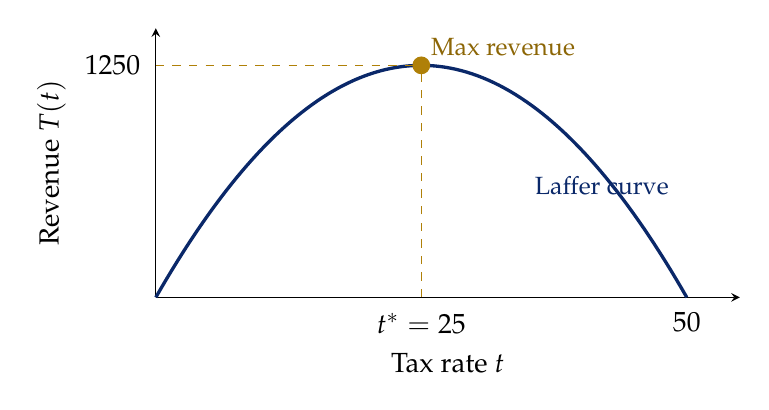
\begin{tikzpicture}
\begin{axis}[
  width=9cm, height=5cm,
  axis lines=left,
  xlabel={Tax rate $t$},
  ylabel={Revenue $T(t)$},
  xmin=0, xmax=55, ymin=0, ymax=1450,
  xtick={25,50},
  xticklabels={$t^*=25$, $50$},
  ytick={1250},
  yticklabels={$1250$},
  tick style={draw=none},
  grid=none,
  clip=false,
]
  \addplot[navy, very thick, domain=0:50, samples=100]{100*x-2*x^2};
  \addplot[only marks, mark=*, mark size=3pt, gold]
    coordinates{(25,1250)};
  \addplot[gold, dashed, thin] coordinates{(25,0)(25,1250)};
  \addplot[gold, dashed, thin] coordinates{(0,1250)(25,1250)};
  \node[gold!80!black, above right, font=\small] at (axis cs:25,1250)
    {Max revenue};
  \node[navy, font=\small] at (axis cs:42,600){Laffer curve};
\end{axis}
\end{tikzpicture}
\captionof*{figure}{\small Tax revenue rises to $t^*=25$, then falls as the
tax base erodes; revenue is zero at the prohibitive rate $t=50$.}
\end{center}
\end{solbox}

%% ═══════════════════════════════════════════════════════════════════════════
\section*{Summary: Key Results}
\addcontentsline{toc}{section}{Summary: Key Results}
%% ═══════════════════════════════════════════════════════════════════════════

\begin{center}
\begin{tabular}{>{\bfseries\color{navy}}p{4.2cm} p{9.4cm}}
  \toprule
  \rowcolor{tabhead}
  \color{white}\textbf{Result} & \color{white}\textbf{Statement} \\
  \midrule
  Extreme Value Theorem
    & Continuous $f$ on closed bounded $[a,b]$
      attains its global max and min. \\
  \rowcolor{tabeven}
  Fermat's Theorem (FOC)
    & Interior local extremum $\Rightarrow$ $f'(x^*)=0$
      (necessary only). \\
  First Derivative Test
    & Sign change of $f'$: $+\to-$ max; $-\to+$ min;
      no change --- inflection. \\
  \rowcolor{tabeven}
  SOC (sufficient)
    & $f'(x^*)=0$ and $f''(x^*)<0$: local max;
      $f''(x^*)>0$: local min. \\
  Higher-order test
    & When $f''(x^*)=0$, find lowest $n$: odd $\Rightarrow$ inflection;
      even, $-$ $\Rightarrow$ max; even, $+$ $\Rightarrow$ min. \\
  \rowcolor{tabeven}
  Concavity and global max
    & $f$ concave on $I$, $f'(x^*)=0$ $\Rightarrow$ $x^*$ is global max on $I$. \\
  Convexity and global min
    & $f$ convex on $I$, $f'(x^*)=0$ $\Rightarrow$ $x^*$ is global min on $I$. \\
  \rowcolor{tabeven}
  AC min and MC
    & $AC'(q^*)=0 \iff MC(q^*) = AC(q^*)$ \\
  Closed interval method
    & Check all interior critical points \emph{and} both endpoints. \\
  \rowcolor{tabeven}
  Monotone transformation
    & Strictly increasing $g$ preserves argmax:
      $\argmax f = \argmax g(f)$. \\
  Inflection point
    & $f''$ changes sign at $x_0$; $f''(x_0)=0$ is necessary not sufficient. \\
  \rowcolor{tabeven}
  MR--Elasticity
    & $\text{MR} = P\!\left(1+\tfrac{1}{\varepsilon_{Q,P}}\right)$;
      revenue max at $|\varepsilon|=1$. \\
  \bottomrule
\end{tabular}
\end{center}

\begin{keybox}{References}
\begin{itemize}
  \item \textbf{Primary}: Chiang \& Wainwright,
        \textit{Fundamental Methods of Mathematical Economics}, 4th ed.,
        McGraw-Hill, 2005. Chapters 9--10.
  \item \textbf{Supplementary}: Hoy, Livernois, McKenna, Rees \& Stengos,
        \textit{Mathematics for Economics}, 3rd ed., MIT Press, 2011.
        Chapters 5, 10.
  \item \textbf{Supplementary}: Simon \& Blume,
        \textit{Mathematics for Economists}, Norton, 1994. Chapters 3--4, 13.
\end{itemize}
\end{keybox}

\vspace{1cm}
\begin{center}
  \textcolor{slate}{\rule{0.5\linewidth}{0.5pt}}\\[6pt]
  \textcolor{slate}{\small\itshape
    End of Notes --- ECON 320 Optimisation of Single-Variable Functions
    --- May 2026}
\end{center}

\end{document}